\title{CS254 Algorithmic Graph Theory - Lecture Notes}
\author{Based on lectures by Prof. Maxim Sviridenko and Dr. Justin Ward \\ Typeset by Alex J. Best}
\date{\today}

\documentclass{article}
\usepackage{amsfonts}
\usepackage{amsmath}
\usepackage{amssymb}
\usepackage{amsthm}
\usepackage{tikz}
\usepackage{hyperref}
\usetikzlibrary{arrows}


\newtheorem*{thm}{Theorem}
\newtheorem*{lem}{Lemma}
\newtheorem*{cor}{Corollary}
\newtheorem*{prop}{Proposition}
\theoremstyle{definition}
\newtheorem*{defn}{Definition}
\newtheorem*{defns}{Definitions}
\newtheorem*{ex}{Example}
\newtheorem*{exer}{Exercise}
\newtheorem*{rem}{Remark}
\newtheorem*{nota}{Notation}
\newtheorem*{alg}{Algorithm}

\newcommand{\ZZ}{\mathbb{Z}}
\newcommand{\QQ}{\mathbb{Q}}
\newcommand{\NN}{\mathbb{N}}
\newcommand{\RR}{\mathbb{R}}
\newcommand{\x}{\mathbf{x}}
\newcommand{\X}{\mathcal{X}}
\newcommand{\I}{\mathcal{I}}
\newcommand{\J}{\mathcal{J}}
\newcommand{\B}{\mathcal{B}}

\newcommand{\bb}[1]{\mathbb{#1}}
\DeclareMathOperator{\wt}{wt}
\DeclareMathOperator{\depth}{depth}
\DeclareMathOperator{\OPT}{OPT}
\DeclareMathOperator{\ecr}{ecr}

%TODO List:
%- Fix formatting on \lceil type bits


\setcounter{tocdepth}{3}

\begin{document}
\maketitle
\tableofcontents
\section*{Introduction}
These are lecture notes I typeset for CS254 Algorithmic Graph Theory in 2013, they are currently full of gaps, mistakes, wrong statements, notation abuse and lots of other badness.
However they might be useful to someone, despite the fact they lack any pictures at present.
Thanks are due to Julian ``Boolean'' Bhardwaj and Rosie Nasrin for telling me I'm wrong.
If you find anything else that can be improved send me an email at a.j.best@warwick.ac.uk, thanks.
\clearpage

\section{Graphs}
\marginpar{Lecture 1}
\begin{defn}
A \emph{graph} $G$ is an ordered pair $(V(G),E(G))$ consisting of a set $V(G)$ of vertices and a set $E(g)$ of edges.
Each edge $e\in E(G)$ is associated with a pair of vertices $\{u,v\}$.
We will say that $u,v$ are endpoints of $e$.
We also say $u,v$ are incident to $e$ and vice versa.
\end{defn}

\begin{defn}
Two vertices which are incident with a common edge are called \emph{adjacent} (or sometimes \emph{neighbours}). \\
Two or more edges with the same pair of endpoints are said to be \emph{parallel}.
\end{defn}

\begin{defn}
A \emph{simple} graph is one without parallel edges.
\end{defn}

\begin{nota}
By convention, $G$ will denote a graph, $n$ and $m$ will be the number of vertices $|V(G)|$ and the number of edges $|E(G)|$ respectively.
\end{nota}

\section{Special graphs}
\begin{defn}
A \emph{complete} graph is a simple graph in which every two vertices are adjacent. \\
Such a graph on $n$ vertices is denoted $K_n$.
\end{defn}
\begin{center}
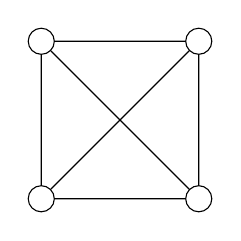
\begin{tikzpicture}
  \node[draw,circle] (G-1) at (0,0) {};
  \node[draw,circle] (G-2) at (0,2) {};
  \node[draw,circle] (G-3) at (2,2) {};
  \node[draw,circle] (G-4) at (2,0) {};
  \draw (G-1) -- (G-2) -- (G-3) -- (G-4) -- (G-1) -- (G-3) -- (G-2) -- (G-4) ;
\end{tikzpicture}
\end{center}

We can see that $|E(K_n)| = \frac{n(n-1)}{2}$.
\begin{defn}
A graph $G=(V,E)$ is called empty if $E=\emptyset$.
\end{defn}

\begin{defn}
A graph is called \emph{bipartite} is its vertex set can be partitioned into two subsets $X$ and $Y$ so that every edge has one endpoint in $X$ and one in $Y$.
\end{defn}

\begin{ex}
The set of all (monogamous) people can be represented by a graph with edges joining married couples, this graph is bipartite.
\end{ex}

We will call $X,Y$ the parts of the graph.
So a bipartite graph is often denoted as $G = (X,Y,E)$.
\begin{nota}
We write $K_{m,n}$ for the complete bipartite graph with $|X| = m,\ |Y| = n$ and $E$ containing all edges between $X$ and $Y$.
\end{nota}

\begin{defn}
The graph $K_{1,n}$ is often called a star.
\end{defn}
\begin{center}
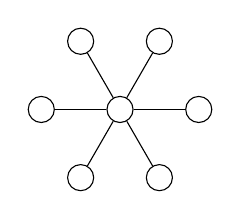
\begin{tikzpicture}
  \node[draw,circle] (G-1) at (0,0) {};
  \node[draw,circle] (G-2) at (1,0) {};
  \node[draw,circle] (G-3) at (0.5,0.866) {};
  \node[draw,circle] (G-4) at (-0.5,0.866) {};
  \node[draw,circle] (G-5) at (-1,0) {};
  \node[draw,circle] (G-6) at (-0.5,-0.866) {};
  \node[draw,circle] (G-7) at (0.5,-0.866) {};
  \draw (G-1) -- (G-2);
  \draw (G-1) -- (G-3);
  \draw (G-1) -- (G-4);
  \draw (G-1) -- (G-5);
  \draw (G-1) -- (G-6);
  \draw (G-1) -- (G-7);
\end{tikzpicture}
\end{center}
%TODO: pictures

\begin{defn}
A \emph{path} is a simple graph whose vertices can be rearranged into a linear sequence in such a way that two adjacent vertices are always consecutive in the sequence and vice versa, non-adjacent vertices are non-consecutive.
Such a graph on $n$ vertices is often denoted $P_n$.
\end{defn}
\begin{center}
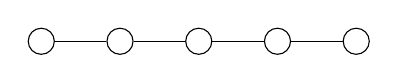
\begin{tikzpicture}
  \node[draw,circle] (G-1) at (0,0) {};
  \node[draw,circle] (G-2) at (1,0) {};
  \node[draw,circle] (G-3) at (2,0) {};
  \node[draw,circle] (G-4) at (3,0) {};
  \node[draw,circle] (G-5) at (4,0) {};
  \draw (G-1) -- (G-2) -- (G-3) -- (G-4) -- (G-5);
\end{tikzpicture}
\end{center}

\begin{defn}
A \emph{cycle} on $n$ vertices is a graph defined in the same way but with a cyclic sequence of vertices.
\end{defn}
\begin{center}
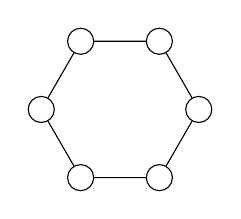
\begin{tikzpicture}
  \node[draw,circle] (G-1) at (1,0) {};
  \node[draw,circle] (G-2) at (0.5,0.866) {};
  \node[draw,circle] (G-3) at (-0.5,0.866) {};
  \node[draw,circle] (G-4) at (-1,0) {};
  \node[draw,circle] (G-5) at (-0.5,-0.866) {};
  \node[draw,circle] (G-6) at (0.5,-0.866) {};
  \draw (G-1) -- (G-2) -- (G-3) -- (G-4)  -- (G-5)  -- (G-6) -- (G-1);
\end{tikzpicture}
\end{center}

\begin{nota}
The length of a path or cycle is the number of its edges. A path or cycle of length $k$ is often called a $k$-path of $k$-cycle.
\end{nota}
\begin{center}
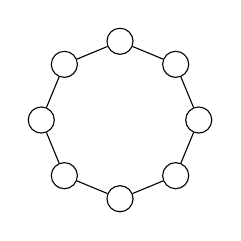
\begin{tikzpicture}
  \node[draw,circle] (G-1) at (1,0) {};
  \node[draw,circle] (G-2) at (0.707,0.707) {};
  \node[draw,circle] (G-3) at (0,1) {};
  \node[draw,circle] (G-4) at (-0.707,0.707) {};
  \node[draw,circle] (G-5) at (-1,0) {};
  \node[draw,circle] (G-6) at (-0.707,-0.707) {};
  \node[draw,circle] (G-7) at (0,-1) {};
  \node[draw,circle] (G-8) at (0.707,-0.707) {};
  \draw (G-1) -- (G-2) -- (G-3) -- (G-4)  -- (G-5)  -- (G-6) -- (G-7) -- (G-8) -- (G-1);
\end{tikzpicture}
\end{center}

\section{Adjacency and incidence matrices}

\begin{defn}
The \emph{incidence matrix} of $G = (V,E)$ when $|V| = m$ and $|E| = n$ is the $m\times n$ matrix $M_G = (m_{ve})$ where $m_{ve}$ is the number of times that vertex $v$ and $e$ are incident ($m_{ve} \in \{0, 1\}$).
\end{defn}

\begin{ex}
$$G=
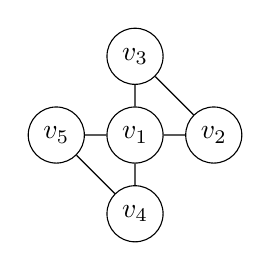
\begin{tikzpicture}[baseline=-0.5ex]
  \node[draw,circle] (G-1) at (0,0) {$v_1$};
  \node[draw,circle] (G-2) at (1,0) {$v_2$};
  \node[draw,circle] (G-3) at (0,1) {$v_3$};
  \node[draw,circle] (G-4) at (0,-1) {$v_4$};
  \node[draw,circle] (G-5) at (-1,0) {$v_5$};
  \draw (G-1) -- (G-2) -- (G-3) -- (G-1) -- (G-4) -- (G-5) -- (G-1);
\end{tikzpicture}
\text{ has incidence matrix }
\begin{pmatrix}
1 & 1 & 0 & 1 & 1 & 0 \\
1 & 0 & 1 & 0 & 0 & 0 \\
0 & 1 & 1 & 0 & 0 & 0 \\
0 & 0 & 0 & 1 & 0 & 1 \\
0 & 0 & 0 & 0 & 1 & 1
\end{pmatrix} = M_{G}$$
\end{ex}

\begin{defn}
The \emph{adjacency matrix} of $G = (V,E)$ when $|V| = m$ is the $m\times m$ matrix $A_G = (a_{uv})$ where $a_{uv}$ is the number of edges joining $u$ and $v$.
\end{defn}

\begin{ex}
$$K_3 = 
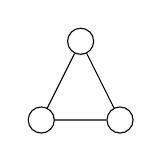
\begin{tikzpicture}[baseline=2ex]
  \node[draw,circle] (G-1) at (-0.5,0) {};
  \node[draw,circle] (G-2) at (0.5,0) {};
  \node[draw,circle] (G-3) at (0,1) {};
  \draw (G-1) -- (G-2) -- (G-3) -- (G-1);
\end{tikzpicture}
\text{ has adjacency matrix }
\begin{pmatrix}
0 && 1 && 1 \\
1 && 0 && 1 \\
1 && 1 && 0 
\end{pmatrix} = A_{K_{3}}$$
\end{ex}

\begin{defn}
An \emph{adjacency list} is a list $(N(v),v\in V)$ used to represent matrices, $N(v)$ is the set of neighbours of $v$ in arbitrary order.
\end{defn}

\section{Vertex degrees}

\begin{defn}
The \emph{degree} of a vertex $v$ in a graph $G$ is denoted $d_G(v)$ or $d_v$ and is the number of edges of $G$ incident with $v$.
\end{defn}

\begin{thm}[Handshake lemma]
For any graph
\begin{equation} \label{eq:hand}
\sum_{v\in V}d_v = 2|E|
\end{equation}
\end{thm}

\begin{thm}
In any graph, the number of vertices of odd degree is even.
\end{thm}

\begin{proof}
Consider the equation \ref{eq:hand} modulo 2.
We have degree of each vertex $d_v \equiv$ 1 if $d_v$ is odd, or 0 is $d_v$ is even.
Therefore the left hand side of \ref{eq:hand} is congruent to the number of vertices of odd degree and the RHS is 0.
Therefore the number of vertices of odd degree is congruent to 0 mod 2.
\end{proof}

\begin{defn}
A graph $G$ is called \emph{$k$-regular} if $d_G(v) = k$ for all $v\in V(G)$.
A graph is \emph{regular} if it is $k$-regular for some $k$.
\end{defn}

\begin{ex}
$K_n$ is $(n-1)$-regular. \\
$C_n$ is $2$-regular. \\
$P_n$ is not regular. \\
\end{ex}

\marginpar{Lecture 2}

\begin{thm}
Let $G=(X,Y,E)$ be a bipartite graph without isolated vertices s.t. $d_x\geq d_y$ for all $x\in X$ and $y\in Y$ s.t. $(x,y)\in E$.
Then $|X| \leq |Y|$ with equality iff $d_x = d_y \forall (x,y)\in E$ .
\end{thm}

\begin{proof}
Take the adjacency matrix $B$.
Define the matrix $B'$ by dividing each row of $B$ corresponding to vertex $u$ by $d_u$.
Consider one column sum corresponding to $y\in Y$.
$$\sum_{x\in X} b'_{xy} = \sum_{(x,y)\in E} \frac{1}{d_x} = \frac{d_y}{d_x} \leq 1$$
Therefore $|X|=\sum_{x\in X}\sum_{y\in Y,(x,y)\in E} \frac{1}{d_x}$
$$=\sum_{x\in X, y\in Y}\sum_{(x,y)\in E} \frac{1}{d_x} \leq \sum_{x\in X, y\in Y}^{(x,y)\in E} \frac{1}{d_y}$$
$$=\sum_{y\in Y} \sum_{x\in X,(x,y)\in E} \frac{1}{d_y} = |Y|$$
If $|X|=|Y|$, then the middle inequality must be an inequality implying that $d_x=d_y$ for all $(x,y)\in E$.
\end{proof}

\section{Isomorphisms}

\begin{defn}
Two graphs $G$ and $H$ are \emph{isomorphic}, written $G\cong H$, if there is a bijection $\Theta\colon V(G) \to V(H)$ such that $(u,v)\in E$ iff $(\Theta(u),\Theta(v))\in E(H)$.
\end{defn}

\begin{ex}
$$
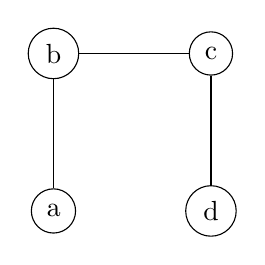
\begin{tikzpicture}[baseline=5.5ex]
  \node[draw,circle] (G-1) at (0,0) {a};
  \node[draw,circle] (G-2) at (0,2) {b};
  \node[draw,circle] (G-3) at (2,2) {c};
  \node[draw,circle] (G-4) at (2,0) {d};
  \draw (G-1) -- (G-2) -- (G-3) -- (G-4);
\end{tikzpicture}\cong
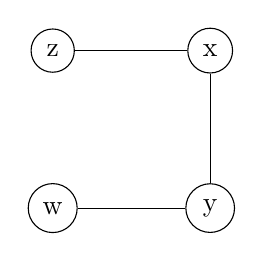
\begin{tikzpicture}[baseline=5.5ex]
  \node[draw,circle] (G-1) at (0,0) {w};
  \node[draw,circle] (G-2) at (0,2) {z};
  \node[draw,circle] (G-3) at (2,2) {x};
  \node[draw,circle] (G-4) at (2,0) {y};
  \draw (G-1) -- (G-4) -- (G-3) -- (G-2);
\end{tikzpicture}$$
%TODO: Examples
\end{ex}

\begin{rem}
\begin{itemize}
\item The mapping $\Theta$ is not unique.
\item Isomorphic graphs have the same number of vertices and edges.
\item Up to isomorphism there is only one complete graph on $n$ vertices denoted $K_n$.
So $K_n$ is a class of graphs that are all isomorphic to each other.
\item The same as above goes for each of $K_{m,n},\ P_n,\ C_n$.
\end{itemize}
\end{rem}

\section{Directed graphs}

\begin{defns}
In a graph $G= (V,E)$ a \emph{walk} from a starting vertex $v_0$ to a destination vertex $v_n$ is a sequence
$$W=\langle v_0,e_1,v_1,e_2,\ldots,e_n,v_n\rangle\text{ s.t. }e_i=(v_{i-1},v_i)$$
The \emph{length} of the walk is the number of edges in the sequence $W$.
A \emph{closed walk} has the same starting and ending vertices.
A \emph{path} is a walk where every vertex appears at most once.\\
The \emph{distance} $d(s,t)$ between a vertex $s$ and a vertex $t$ in a graph $G$ is the length of the shortest path between $s$ and $t$ (if one exists) and $d(s,t)=+\infty$ otherwise.\\
A \emph{weighted graph} $G= (V,E,\omega)$ is a graph and a function $\omega\colon E\to \RR$ assigning weights to edges.
\end{defns}

We now define some problems that drive our study of algorithms in graph theory.
\paragraph{Problem 1}
Given an edge weighted graph $G=(V,E,\omega)$.
Find a shortest path between $s$ and $t$ (length is the sum of the edge weights).

\paragraph{Problem 2}
Minimum-weight spanning tree:
Given an undirected graph $G=(V,E,\omega)$ find an acyclic connected subgraph of $G$ of smallest weight.

\paragraph{Problem 3}
Travelling salesman problem:
We are given a complete weighted graph $G$.
Find a cycle that visits every vertex exactly once and minimises its length.

\paragraph{Problem 4}
Maximum flow problem:
You have a directed graph $G$ representing a system of pipes, each pipe has a capacity.
We are given also the source $S$ and the sink $T$, $S,T\in V(G)$.
How much water can we pump through the network per time unit?

\begin{defn}
A \emph{leaf} is a vertex of degree one.
\end{defn}

\begin{prop}
Every tree $T$ has at least two leaves.
\end{prop}

\begin{proof}
Consider $P=\langle v_1,\ldots,v_k\rangle$ a path of maximum length in $T$.
Consider $v_1$ if $v_1$ has degree more than one then we can either extend the path or $T$ is not acyclic.
\end{proof}

\marginpar{Lecture 3}

\begin{cor}
If the degree of each node in $G$ is $\ge 2$ then $G$ has a cycle.
\end{cor}

\begin{prop}
Each tree has exactly $|V| -1$ edges.
\end{prop}

\begin{proof}
\lbrack By induction\rbrack
\end{proof}

\begin{defns}
An acyclic graph is called a \emph{forest}.\\
A \emph{connected component} of $G$ is a maximal connected subgraph of $G$.
Let $c(G)$ be the number of connected components of $G$. %0th betti number
\end{defns}

\begin{cor}
Any graph on $n$ vertices has at least $n-c(G)$ edges.
\end{cor}

\begin{prop}
If $G$ is a simple graph with $n$ vertices then
$$|E(G)| \le \frac{(n-k)(n-k+1)}{2} \text{ where }k=c(G)$$
\end{prop}

\begin{proof}
Let $c_1,\ldots,c_k$ be the connected components of $G$, i.e. $c_i=(V_i,E_i)$ and $E(G) = \bigcup_{i=1}^k E_i,\ V=\bigcup_{i=1}^k V_i,\ n=|V|$.
Then $n=\sum_{i=1}^k n_i$ and $n_i \ge 1$.
Obviously $|E(G_i)| \le \frac{n_i^2 -n_i}{2}$.
Thus $|E(G)| \le \sum_{i=1}^k \frac{n_i^2-n_i}{2}$.
The maximum of RHS occurs when $|C_1| = |C_2| = \ldots = |C_{k-1}| = 1$ and $|C_k| = n-k +1$. \\
Assume the contrary that the maximum occurs when $c_i = k$, and $c_j = k_s$ where $r\ge s \ge 2$.
Then $|E(c_i)| + |E(c_j)| = \frac{r^2 + s^2 - r -s}{2}$.
But is $c_i = k_{r+1}$ and $c_j = k_{s-1}$, then we have $\frac{(r+1)^2 + (s-1)^2 - (r+1) -(s-1)}{2}$ edges.
We get a contradiction since $(r+1)^2 + (s-1)^2 > r^2 + s^2$.
\end{proof}

\begin{defn}
A \emph{cut-edge} is an edge whose removal increases the number of connected components.
\end{defn}

\begin{thm}
Let $T$ be a graph with $n$ vertices, then the following statements are equivalent:
\begin{enumerate}
\item $T$ is a tree.
\item $T$ contains no cycles and has $(n-1)$ edges.
\item $T$ is connected and has $(n-1)$ edges.
\item $T$ is connected and every edge is a cut-edge.
\item Any two vertices of $T$ are connected by exactly one path.
\item $T$ contains no cycles and for any new edges the graph $T + e$ has exactly one cycle.
\end{enumerate}
\end{thm}

\begin{proof}
$(1\implies 2)$ Previous proposition and definition of tree. \\
$(2\implies 3)$ Suppose $T$ has $k$ connected components.
Then each component must be a tree (because they have no cycles) therefore $T$ must contain $n-k$ edges, exactly $\implies k=1$. \\
$(3\implies 4)$ Let $e$ be an edges of $T$.
Since $T\setminus e$ has $n-2$ edges by one of the corollaries, we must have $c(T)\ge 2$. \\
$(4\implies 5)$ (By contradiction) Suppose $x$ and $y$ are two vertices of tress $T$ that have two different paths, say $p_1$ and $p_2$ connecting them.
Let $u$ be the first vertex where the paths diverge and let $v$ be the first vertex where the paths meet again.
Any edge of the cycle containing $u$ and $v$ is not a cut edge which contradicts (4). \\
$(5\implies 6)$ $T$ contains no cycles otherwise we would have two paths between $x,y\in$ cycle.
If we add an edge $e= (u,v)$ we will create a cycle since $T$ contains a path between $u$ and $v$. If $T+e$ contains two cycles then both cycles must contain $e$.
$u,v$ have two different paths containing them in $T$ is a contradiction. \\
$(6\implies 1)$ \lbrack By definition \rbrack \\
\end{proof}

\section{Huffman Trees and Optimal Prefix Codes}

\begin{defns}
A \emph{binary code} is an assignment of symbols or other meanings to a set of bitstrings.\\
A \emph{prefix code} is a binary code with the property that no codeword is an initial substring of any other codeword.
\end{defns}

This allows for transmission without confusion.

\begin{ex}
A prefix code for an alphabet: construct a binary tree with a leaf corresponding to a letter of your alphabet, every left-hand edge is labelled by 0 and right-hand edge is labelled by 1.
%TODO: Pictures!
\end{ex}

\marginpar{Lecture 4}

\begin{defns}
Assume we have a code.
Each codeword has a length $l_c$ and each symbol has its frequency $p_c$.
The \emph{code efficiency} is then$\sum p_cl_c$. \\
Let $T$ be a binary tree with leaves $s_1,\ldots,s_l$ such that each leaf $s_i$ is assigned weight $w_i$.\\
The \emph{average weighted depth} of the binary tree $T$ is $\wt(T) = \sum_{i=1}^l\depth(s_i)w_i$ where depth is the number of edges to the root.
\end{defns}

\begin{alg}[Constructing Huffman Prefix Codes]~\\
\textbf{Input} $s_1,\ldots,s_l$ of symbols and a list of $w_1,\ldots,w_l$ of weights $w_i$ corresponding to $s_i$.\\
\textbf{Output} A binary tree representing a prefix code for a set of symbols whose codewords have minimum average weighted length.\\
Initialise $F$ to be a forest of isolated vertices, labelled $s_1,\ldots,s_l$ with respective weights $w_1,\ldots, w_l$. \\
For $i=1$ to $l-1$ Choose two trees $T$ and $T'$ from the forest of smallest weights.\\
Create a binary tree by adding a new vertex with $T$ as a child on the left and $T'$ a child on the right. Label the edges to these new child trees 0 and 1 respectively. \\
Assign to the new tree the weight $\wt(T)+\wt(T')$. \\
Replace $T$ and $T'$ in $F$ by the new tree. \\
When finished return $F$.
\end{alg}

\begin{ex}
%TODO:examples
\end{ex}

\begin{lem}
If the leaves of a binary tree are assigned weights and if each internal vertex (node) is assigned a weight equal to the sum of its children's weights, then the tree's average weighted depth equals the sum of the weights of its internal (non-leaf) vertices.
\end{lem}

\begin{proof}
In assignments.
\end{proof}

\begin{thm}
For a given list of weights $w_1,\ldots,w_l$ a Huffman tree has the smallest average weighted depth among all binary trees whose leaves are assigned these weights.
\end{thm}

\begin{proof}
Induction on $l$.
Let $T$ be the Huffman tree.
\textbf{Base case} $l=2$. Then $\wt(T) = w_1 + w_2$, because $T$ is the only tree on 3 vertices.
\textbf{Inductive step} Assume that for some $l\ge 2$ the Huffman algorithm produces a Huffman tree of minimum average weighted depth for any list of $l$ weights. \\
We are given $w_1\le w_2\le \ldots\le w_{l+1}$. The Huffman tree $H$ that is constructed by the algorithm consists of the Huffman tree $\bar{H}$ for the weights $w_1+w_2,w_3,\ldots,w_{l+1}$ where the leaf with weight $w_1+w_2$ is replaced by a tree with two children of weights $w_1$ and $w_2$.
By the previous lemma, we know $\wt(H) = \wt(\bar{H}) + w_1 + w_2$.
By the inductive hypothesis, $\bar{H}$ is optimal among all binary trees whose leaves are assigned weights  $w_1+w_2,w_3,\ldots,w_{l+1}$. \\
Suppose $T^*$ is an optimal binary tree for the weights $w_1,\ldots,w_{l+1}$.
Let $x$ be an internal vertex of $T^*$ of greatest depth and suppose $y$ and $z$ are its left child and right child respectively. Without loss of generality, $y$ and $z$ have weights $w_1$ and $w_2$ otherwise we can swap their weights with $w_1$ and $w_2$ and produce a tree with the same or better weights.
Delete $y$ and $z$ from $T^*$ and call this tree $\bar{T}$, we have $\wt(T^*) = \wt(\bar{T}) + w_1 + w_2$. We also know that $\wt(\bar{T}) \ge \wt(\bar{H})\implies \wt(T^*)\ge \wt(H)$.
\end{proof}

\marginpar{Lecture 5}

\begin{defn}
Given trees $T=(V,E)$ and $T' = (V,E')$ we say $T=T'$ if $E = E'$.
\end{defn}

\begin{ex}
%TODO:examples of unequal but isomorphic trees.
\end{ex}

\begin{thm}[Cayley's Formula]
The number of $n$ vertex labelled trees is $n^{n-2}$.
\end{thm}

\begin{defn}
A \emph{Pr\"ufer sequence} of length $n-2$ for $n\ge 2$ is any sequence of integers between 1 and $n$ with repetitions allowed.
There are $n^{n-2}$ of these.
\end{defn}

\begin{alg}~\\
\textbf{Input} An $n$-vertex tree.\\
\textbf{Output} A Pr\"ufer sequence of length $n-2$.\\
Initialise $T$ to be a given tree \\
For $i=1$ to $n-2$ \\
\indent Let $v$ be the vertex of degree 1 with smallest label.\\
\indent Let $s_i$ be the only neighbour of $v$.\\
\indent Define $T = T\setminus v$\\
Return the sequence $\langle s_1,\ldots,s_{n-2}\rangle$
\end{alg}

\begin{ex}
%TODO:yet more examples
\end{ex}

\begin{prop}
Let $d_k$ be the number of occurrences of the number $k$ in a Pr\"ufer encoding sequence for a labelled tree $T$.
Then the degree of $k$ in $T$ is $d_k+1$.
\end{prop}

\begin{proof}
By induction: \\
The assertion is true for any tree on 3 vertices since the Pr\"ufer sequence consists of a single label of the vertex of degree 2. \\
Assume the assertion is true for all labelled trees on $n$ vertices for some $n\ge 3$.\\
Let $T$ be a labelled tree on $n+1$ vertices.
Let $v$ be a leaf with smallest label $l(v)$.
Let $w$ be a neighbour of $v$.
Then the Pr\"ufer sequence $S$ for $T$ consists of $l(w)$ followed by $S^*$, the Pr\"ufer sequence of $T^* = T\setminus v$. \\
Now by the inductive hypothesis, for each $u\in T^*$ the number of occurrences of $l(W)$ in $S^*$ is $d_{T^*}(u)-1$.
But for all $u\ne w$ the number of occurrences of the label $l(u)$ in $S^*$ is the same as in $S$, and $d_T(u)=d_{T^*}(u)$.
Moreover, $d_T(w) = d_{T^*}(w) + 1$ and $l(w)$ has one more occurrence in $S$ than in $S^*$.
\end{proof}

\begin{alg}[for Pr\"ufer decoding]~\\
\textbf{Input} A Pr\"ufer sequence of length $n-2$.\\
\textbf{Output} An $n$-vertex labelled tree.\\
Initialise list $P$ as a Pr\"ufer input sequence. \\
Initialise list $L$ as $1,\ldots, n$. \\
Initialise $F$ (forest) as $n$ isolated vertices labelled $1,\ldots, n$. \\
For $i=1,\ldots, n-2$ \\
\indent Let $k$ be the smallest number in the list $L$ that is not in the list $P$ (Exists as $P<L$). \\
\indent Let $j$ be the first number in the list $P$. \\
\indent Add an edge $(k,j)$ to the forest $F$.\\
\indent Remove $k$ from $L$.\\
\indent Remove the first occurrence of $j$ from $P$.\\
Add an edge joining the two vertices labelled with two remaining numbers in the list $L$.\\
Return $F$ with its vertex labelling.
\end{alg}

\marginpar{Lecture 6}

\begin{prop}
The decoding procedure defines a function $f'\colon P_{n-2} \to T_n$.
\end{prop}

\begin{proof}
$f'$ that corresponds to the decoding algorithm maps a sequence to a graph.
We need to show that this graph is a tree. \\
Proceed by induction: \\
\textbf{Base case} For $n=2$, the sequence is empty and the algorithm produces a single edge. \\
\textbf{Inductive step} Assume that the claim is true for some $n\ge 2$.
Consider a Pr\"ufer sequence on $\langle p_1,\ldots,p_{n-1}\rangle$ and a set of vertices $\{1,2,\ldots,n+1\}$.
The first iteration draws an edge from $b$ to $p_1$, where $b$ is the smallest index not appearing among the $p_i$'s.
None of the $n-1$ edges that are produced in iterations $2,\ldots,n$ will be incident with $b$.
Thus, continuing the procedure from iteration 2 is equivalent to applying the procedure to the Pr\"ufer sequence $\langle p_2,\ldots,p_{n-1}\rangle$ for the set of vertices $X = \{1,\ldots,n+1\}\setminus b$.
By induction we will provide a tree on $X$.
This tree plus an edge of $p_1$ forms a tree on $\{1,\ldots,n+1\}$.
\end{proof}

\begin{exer}
Prove that different elements of $P_{n-2}$ are mapped into different trees and conversely.
\end{exer}

\section{Catalan numbers}

Let $b_n$ be the number of unlabelled binary trees on $n$ vertices.
By convention we define $b_0 = 1$.
Trivially $b_1 = 1$.
For $n>1$ a binary tree on $n$ vertices could have $j$ vertices on the left and $n-1-j$ vertices on the right, for $j=0,\ldots,n-1$. \\
There are $b_jb_{n-1-j}$ different ways to pair up such subtrees.
Therefore we have
$$b_n =\sum_{j=0}^{n-1} b_jb_{n-1-j}$$

\begin{thm}
$$b_n = \frac{1}{n+1}\binom{2n}{n}$$
\end{thm}

So $b_2=2,\ b_3=5$.

\begin{ex}
Consider a sequence of $n$ parenthesis that are correctly matched.
For $n=2$ we have $\{(()),\ ()()\}$.
For $n=3$ we have $\{((())),\ (())(),\ (()()),\ ()(()),\ ()()()\}$.
The number such expressions is $b_n$ -- the Catalan numbers.
\end{ex}

\section{Connectivity}

\begin{defn}
A \emph{vertex-cut} in a graph is a set of vertices $V$ such that $G\setminus V$ has more connected components than $G$. \\
We often write $k$-connectivity to mean $k$-vertex connectivity, $k$-edge connectivity is a similarly defined but different concept.
\end{defn}

When $k=1$ a tree is an example of a one-edge connected graph.\\
When $k=2$ a cycle is an example of a two-vertex connected graph.

\begin{prop}
Let $e$ be any edge of a $k$-connected graph for $k\ge 3$.
Then graph $G\setminus e$ is $(k-1)$-connected.
\end{prop}

\begin{proof}
Let $W=\{w_1,\ldots,w_{k-2}\}$ be any set of $k-2$ vertices and $G\setminus e$ and let $x$ and $y$ be any two different vertices in $(G\setminus e)\setminus W$.
It is enough to show that there is an $x$-$y$ walk in $(G\setminus e)\setminus W$. \\
If $e=(u,v)$ and $u\in W$ or $v\in W$, then $G\setminus W = (G\setminus e) \setminus W$ and we know that $G\setminus W$ has a path between $x$ and $y$ since $G$ is $k$-connected. \\
Assume that $u\not\in W$ and $v\not\in W$. \\
\textbf{Case 1} The vertices $x,y$ are the endpoints of $e$.
Graph $G$ has at least $k+1$ vertices.
Since $G$ is $k$-connected. 
So $\exists z\in G\setminus\{W\cup\{x,y\}\}$.
Since $G$ is $k$-connected, there exists an $x$-$z$ path $P_1$ in the graph $G\setminus W\cup\{x\}$.
These paths do not contain $e$.
Therefore $(P_1,P_2)$ is an $x$-$y$ path in $(G\setminus e)\setminus W$. \\
\textbf{Case 2} One of the vertices $x$ or $y$, say $x$ is not an endpoint of $e$.
Let $u$ be an endpoint of $e$ that is different from $y$.
Since $G$ is $k$-connected, the graph $G' = G\setminus W\cup\{u\}$ is connected and there is an $x$-$y$ path $P$ in $G'$.
$G'$ does not contain $e$.
Therefore there is an $x$-$y$ path in $(G\setminus e)\setminus W$.
\end{proof}


\marginpar{Lecture 7}
\begin{cor}
Let $G$ be a $k$-connected graph and let $D$ be any set of $m$ edges of $G$ for $m\le k-1$.
Then the graph $G\setminus D$ is $(k-m)$-connected.
\end{cor}

\begin{defn}
A collection of paths in $G$ is said to be \emph{internally disjoint} if no two paths in the collection have an internal node in common.
\end{defn}

\begin{thm}[Whitney's 2-connected characterisation]
Let $G$ be a connected graph with $|V(G)| \ge 3$.
Then $G$ is 2-connected $\iff$ for each pair of vertices in $G$, there are two internally disjoint paths between them.
\end{thm}

\begin{proof}
($\Leftarrow$) Suppose $G$ is not 2-connected.
Then there is a cut-vertex $v\in V(G)$.
Therefore $\exists x,y\in G\setminus v$ such that there is no $x$-$y$ path in $V\setminus v$.
Therefore $v$ must be an internal vertex of any $x$-$y$ path in $G$. \\
%TODO: possible diagram
($\Rightarrow$) Suppose $G$ is 2-connected, and let $x$ and $y$ be any two vertices of $G$.
Induction on $d(x,y)$.
If $\exists e=(x,y)$ then $d(x,y) = 1$.
Also we know that $G\setminus e$ is connected.
Let $P$ be an $x$-$y$ path in $G\setminus e$.
Then $e$ and $f$ are internally disjoint. \\
Assume that the statement is true for any $x',y'$ such that $d(x',y')\le k-1$.
Let $x,y\in V(G)$ and $d(x,y) = k$. \\
Consider a path between $x$ and $y$ of length $k$.
Let $w$ be the vertex on this path immediately preceding $y$ and let $e=(w,y)$.
Since $d(x,w)<k$ we know that there are two internally disjoint paths in $G$, say $P$ and $Q$ connecting $x$ and $w$.
Also, there should be a path $R$ in $G\setminus w$ connecting $x$ and $y$.
Let $z$ be the vertex on $R$ that precedes $y$ and is also on one of the paths $P$ or $Q$ ($z$ could be vertex $x$).
Assume WLOG on $P$. \\
\textbf{Option 1}
Consider two paths constructed as follows: \\
Follow $P$ from $x$ to $z$ and $R$ from $z$ to $y$, call this path 1.
For path 2 we follow $Q$ from $x$ to $w$ and $e$ from $w$ to $y$. \\
\textbf{Option 2}
The first path is as above. \\
The second path follows $Q$ from $x$ to $y$.
\end{proof}

\begin{cor}
$G$ is 2-connected $\iff$ Any two vertices lie on a common cycle.
\end{cor}

\begin{thm}
The following are equivalent:
\begin{enumerate}
\item $G$ is 2-connected.
\item For any two vertices there is a cycle in $G$ containing both of them.
\item For any vertex and any edge of $G$, there is a cycle containing both.
\item For any two edges of $G$, there is a cycle containing both.
\item For any two vertices and one edge, there is a path containing all three.
\item For any three vertices and one edge there is a path containing all four.
\item For any three distinct vertices of $G$, there is a path containing any two of them which does not contain the third.
\end{enumerate}
\end{thm}

\section{Constructing Reliable Networks}

\begin{defns}
A \emph{Whitney-Robbins synthesis} of graph $G$ from a graph $H$ is a sequence of graphs $G_0=H,G_1,\ldots,G_l=G$ and $G_i$ is the result of a path or a cycle addition in $G_{i-1}$ for $i=1,\ldots,l$. \\
A \emph{path addition} in $G$ is the addition of a path between two vertices of $G$, all internal vertices and edges are new. \\
A \emph{cycle addition} in $G$ is the addition of a cycle that has exactly one vertex in common with $G$. \\
If the graph $G_i$ is the result of a path additions only from $H$, then the sequence $G_0,\ldots,G_l$ is called a \emph{Whitney synthesis}.
\end{defns}

\marginpar{Lecture 8}

\begin{lem}
Adding a path to a 2-connected graph keeps it 2-connected.
\end{lem}

\begin{proof}
Consider $u$ and $v\in V(G)$ where $G$ is a 2-connected graph.
We add a path between $u$ and $v$.
To prove that the new graph is 2-connected it is enough to show that there are 2 paths $P_1$ and $P_2$ such that they are internally disjoint and $P_1$ connects $y$ to $u$ and $P_2$ connects $y$ to $v$ for any vertex $y$. \\
We take $Q_1$ and $Q_2$ two internally disjoint paths between $y$ and $u$, and any path $R$ between $y$ and $v$.
Assume that $R$ intersects $Q_1$ or $Q_2$ and $z$ is the latest intersection point.
Without loss of generality $z\in Q_2$.
Choose $Q_1$ and follow $Q_2$ till $z$ and $R$ from $z$ to $v$.
\end{proof}

\begin{thm}
A graph $G$ is 2-connected $\iff$ $G$ is a cycle or a Whitney synthesis from a cycle.
\end{thm}

\begin{proof}
($\Leftarrow$) Let $C=G_0,\ldots,G_l=G$ is a Whitney synthesis.
The cycle is 2-connected, so from the lemma above $G$ is also.\\
($\Rightarrow$) Suppose $G$ is a 2-connected graph and let $C$ be any cycle in $G$.
Let $\mathcal{H}$ be a collection of all subgraphs of $G$ that are Whitney syntheses from a cycle $C$.
The collection $\mathcal{H}$ is non-empty since $c\in\mathcal{H}$.
Let $H^*$ be a graph in $\mathcal{H}$ with maximum number of edges.
Suppose $H^*\ne G$.
The connectedness of $G$ implies that $\exists e=(v,w)\in E_G\setminus E_{H^*}$ such that $v\in V(H^*)$.
The 2-connectedness of $G$ implies that there is a cycle in $G$ that contains $e$.
Also there should be at least one such cycle $C_e$ that contains some other $z\in V(H^*)\setminus v$.
Let $z$ be the first vertex of $c_e$ in $H^*$ after $w$.
The portion on $C_e$ from $v$ to $z$ is a path addition to $H^*$.
Contradiction to maximality of $H^*$.
Therefore $H^* = G$.
\end{proof}

\begin{lem}
Let $H$ be a 2-edge-connected graph.
The graph that results from a path or cycle addition is 2-edge-connected.
\end{lem}

\begin{thm}[Whitney Robbins synthesis]
A graph $G$ is 2-edge connected $\iff$ $G$ is a cycle or a Whitney-Robbins synthesis from a cycle.
\end{thm}

\section{Tutte's Synthesis of 3-connected graphs}
\begin{defn}
The $n$-spoke wheel $W_n$ is a cycle on $n$ vertices and one additional vertex (the centre) connected directly to all vertices of the cycle.
\end{defn}

\begin{thm}[Tutte's Synthesis Theorem]
A graph is 3-connected $\iff$ it is a wheel or can be obtained from a wheel by a sequence of the following two operations:
\begin{enumerate}
\item Adding an edge between 2 non-adjacent vertices
\item Replacing a vertex of degree at least 4 by two new vertices $v^1$ and $v^2$ so that $d(v^1) \ge 3$ and $d(v^2)\ge 3$.
\end{enumerate}
\end{thm}

\paragraph{Problem} Given positive integers $n$ and $k$, find a $k$-connected $n$-vertex graph having the smallest possible number of edges. \\
This has a number of real world applications, most notably in the design of reliable communications networks that use the least possible resources.

\marginpar{Lecture 9}

\begin{prop}
Let $h_k(n)$ denote the minimum number of edges a $k$-connected graph on $n$ vertices must have.
Then $h_k(n) \ge \left[\frac{kn}{2}\right]$. 
($h_1(n) = n-1$).
\end{prop}

\begin{proof}
We know that $2|E(G)| \ge  n\delta_{\text{min}}(G)$ where $\delta_{\text{min}}(G)$ is the minimum degree of $G$.
We also know that $\delta_{\text{min}}(G) \ge K_e(G) \ge K_v(G)$.
Therefore $|E(G)| \ge \left[\frac{nK_v(G)}{2}\right]$.
\end{proof}

We are given a cycle on $n$ vertices $0,1,\ldots,n-1$.
For any two vertices of the cycle the mod $n$ distance between $i$ and $j$ is denoted $|i-j|_n$ is the smaller of the two numbers $|j-i|$ and $n-|j-i|$. \\
We look at a class of graphs that are a possible candidate for the solution to our problem above.

\begin{defn}
We define the class of \emph{Harary graphs} $H_{k,n}$ by starting with $n$ vertices and adding edges in three cases as follows: \\
\textbf{Case 1} $k$ even. \\
Let $k=2r$.
Define an edge $(i,j)$ if $|i-j|_n \le 2$. \\
\textbf{Case 2} $k$ odd, $n$ even. \\
Let $k=2r+1$.
We start with the graph $H_{2r,n}$ and add $\frac{n}{2}$ diameters of the original $n$-cycle, i.e. an edge between $i$ and $i+\frac{n}{2}$.
The total number of edges $rn +\frac{n}{2} = \frac{(2r+1)n}{2} = \frac{kn}{2}$.\\
\textbf{Case 3} $k$ odd, $n$ odd. \\
Let $k = 2r+1$.
Start with $H_{2r,n}$ and add $\frac{n+1}{2}$ quasi-diameters.
Draw an edge from 0 to $\frac{n-1}{2}$ and from 0 to $\frac{n+1}{2}$.
Draw edges from $i$ to $i+\frac{n+1}{2}$ for $i=1,\ldots,\frac{n-3}{2}$.
Then $E(G) = 2n + \frac{n+1}{2} = \frac{(2r+1)n+1}{2} = \left[\frac{kn}{2}\right]$.
\end{defn}

\begin{thm}
The Harary graph $H_{k,n}$ is $k$-connected.
\end{thm}

\begin{proof}
\textbf{Case 1} $k=2r$ \\
Suppose that $2r-1$ vertices $i_1,\ldots,i_{2r-1}$ are deleted from $H_{2r,n}$ and let $x$ and $y$ be any two vertices in $H_{2r,n}\setminus \{i_1,\ldots,i_{2r-1}\}$.
We need to show that there is an $x$-$y$ path in this graph.
We either deleted $\le r-1$ vertices on this section of the cycle from $x$ to $y$ or from $y$ to $x$.
Assume WLOG that we delete $\le r-1$ vertices on the section from $x$ to $y$.
Let $S$ be the remaining vertices.
The deletions create gaps on the path from $x$ to $y$, but each gap is $\le r-1$.
Therefore, there is an edge that connects two vertices neighbouring each gap.
Therefore $x$ and $y$ are connected.
\textbf{Case 2} $k=2r+1$, $n$ is even. \\
Suppose $D$ is a set of $2r$ vertices that are deleted from $H_{2r+1,n}$.
Let $x$ and $y$ be two arbitrary vertices in $H_{2r+1,n}\setminus D$.
%TODO:diagrams
Consider $H_{2r+1}\setminus D$.
The only bad case is $r$-consecutive vertices are deleted (set $A$) between $x$ and $y$ and $r$-consecutive vertices are deleted between $y$ and $x$ (set $B$).
Let $A=\{0,\ldots,a+r-1\}$ and $B=\{0,\ldots,b+r-1\}$, where the addition is modulo $n$.
Let $l = |(b+r)-(a-1)|_n$ and $w = b+r + \lfloor \frac{l}{2}\rfloor$.
The $w$ is halfway between $b+r$ and $a-1$.
Let $z=w+\frac{n}{2}$ i.e. $z$ is halfway between $b+r$ and $a-1$ moving counter-clockwise.
The vertex $w$ is not among those deleted by the definition.
The vertex $z$ is not among those deleted either since $z$ is in the middle of the stretch from $b+r$ to $a-1$, we delete equal pieces of size $r$ from both sides of the stretch and the non-deleted piece is non-empty.
%\textbf{Case 3}
\end{proof}

\marginpar{Lecture 10}

\begin{thm}[Menger]
Let $u,v$ be distinct non-adjacent vertices in a connected graph.
Then the maximum number of internally disjoint $u$-$v$ paths in $G$ equals the minimum number of vertices needed to separate $u$ and $v$.
\end{thm}

\section{Optimal Graph Traversals}

\begin{quotation}
``This question is so banal...'' \\
``Thus you see, most noble Sir, how this type of solution bears little relationship to mathematics, and I do not understand why you expect a     mathematician to produce it, rather than anyone else, for the solution is based on reason alone, and its discovery does not depend on any mathematical principle.'' Euler's thoughts on solving the bridges of K\"onigsberg problem.
\end{quotation}

\begin{defns}
An \emph{Eulerian walk} in a graph $G$ is a walk that contains every edge of the graph exactly once. \\
An \emph{Eulerian tour} is a closed Eulerian walk. \\
An \emph{Eulerian graph} is a graph permitting an Eulerian tour.
\end{defns}

\begin{thm}[Euler]
The following statements are equivalent for a connected graph $G$:
\begin{enumerate}
\item $G$ is Eulerian.
\item The degree of every vertex in $G$ is even.
\item $E(G)$ is the union of the edge sets of a set of edge disjoint cycles in $G$.
\end{enumerate}
\end{thm}

\begin{proof}
($1\Rightarrow 2$) Let $C$ be an Eulerian tour in $G$ and let $v$ be the starting vertex of some transversal of $C$.
The initial edge and the final edge of the transversal contribute 2 towards the degree of $v$ and each time the traversal passes through a vertex a contribution of 2 towards the degree also results. \\
($2\Rightarrow 3$) Since $G$ is connected and every vertex has degree $\ge 2$, $G$ contains a cycle say $C_1$.
If $C_1 = G$, there is nothing to prove.
Otherwise, consider $G_1=G\setminus C_1$.
Thus the graph has at least one non-trivial component (isolated vertices are trivial components).
Each vertex of $G_1$ has even degree.
The connected component must contain a cycle $C_2$.
If $E(G_1) = E(C_2)$, we stop.
Otherwise, $G_2 = G_1\setminus E(C_2)$ and we continue.
In the end, $E(G) = \bigcup_{i=1}^r E(C_i)$ where $r$ is the number of iterations. \\
($3\Rightarrow 1$) Assume that $E(G) = \bigcup_{i=1}^r E(C_i)$ for some edge-disjoint cycles $C_i$ and $G$ is connected.
Start at vertex $v_1\in C_1$ and walk along $C_1$.
Let $T_1 = C_1$.
There must be some vertex $v_2$ of $T_1$ belonging to some other cycle say $C_2'$.
We add $C_2'$ into $T_1$ as follows, walk along $T_1$ from $v_1$ to $v_2$, walk along $C_2'$, after that walk from $v_2$ to $v_1$ along $T_1$.
This defines $T_2$ and we repeat this procedure to obtain the proof.
\end{proof}

\begin{thm}
A connected graph has an open Eulerian trail $\iff$ it has exactly two vertices of odd degree.
\end{thm}

\begin{thm}
The following statements are equivalent for a connected digraph $\bar{G}$.
\begin{enumerate}
\item Digraph $\bar{G}$ is Eulerian.
\item For every vertex $v$, $d^+(v) = d^-(v)$.
\item The edge set of $D$ is the union of edge-sets of edge-disjoint directed cycles in $D$.
\end{enumerate}
\end{thm}

\begin{defns}
A bitstring of length $2^n$ is called a \emph{$(2,n)$-de Bruijn sequence} if each of the $2^n$ possible bitstrings of length $n$ occurs exactly once as a substring, where wraparound is allowed. \\
The \emph{$(2,n)$-de Bruijn digraph}, denoted $D_{2,n}$, consists of $2^{n-1}$ vertices labelled by the bitstrings of length $n-1$ and $2^n$ arcs labelled by the bitstrings of length $n$.
The arc from the vertex $a_1,\ldots,a_{n-1}$ to the vertex $b_2,\ldots,b_n$ is labelled $a_1,b_2,\ldots,b_n$.
\end{defns}

\begin{prop}
The $(2,n)$-de Bruijn digraph $D_{2,n}$ is Eulerian.
\end{prop}

\begin{proof}
Show that the indegree $=$ the out degree.
\end{proof}

\marginpar{Lecture 11}

\begin{defn}
A \emph{postman tour} in a graph $G$ is a closed walk that uses each edge at least once. \\
In an edge weighted graph an \emph{optimal postman tour} is one whose total edge-weight is minimal.
\end{defn}

\begin{alg}[Finding optimal postman tours]~\\
\textbf{Input} A connected edge-weighted graph. \\
\textbf{Output} An optimal postman tour $W$. \\
First find the set of odd degree vertices in $G$, call it $S$. \\
For each pair of odd degree vertices $u$ and $v$ in $S$: \\
\indent Find a shortest path $P$ in $G$ between $u$ and $v$. \\
\indent Let $d_{uv}$ be the length of path $P$. \\
Form a complete graph $K_{|S|}$ on the vertices of $S$.\\
For each edge $e = (u,v)$ in $K_{|S|}$, assign the weight $d_{uv}$ to the edge $e$.\\
Find a minimum weight perfect matching $M$ in $K_{|S|}$.\\
For each edge $e=(u,v)$ of the matching $M$: \\
\indent Let $P_e$ be the corresponding path in $G$ between $u$ and $v$. \\
\indent For each edge $f\in P_e$ add a duplicate copy of $f$ to $G$ including its edge-weight. \\
Let $G^*$ be the Eulerian graph consisting of $G$ and edge duplications defined above.
Note that all vertices of odd degree will have an odd number of edges added.
All vertices of even degree will have an even number of edges added. \\
So to finish we construct an Eulerian tour $W$ in $G^*$.
\end{alg}

\section{Hamiltonian paths and cycles}

\begin{defn}
A \emph{Hamiltonian path (or cycle)} of a graph is a path (resp. cycle) that contains all the vertices of the graph.
\end{defn}

For digraphs the path (or cycle) must be directed.

\begin{thm}[Ore, 1960]
Let $G$ be a simple $n$-vertex undirected graph where $n\ge 3$ such that $d(x) + d(y) \ge n$ for each non-adjacent pair $x,y\in V(G)$.
Then $G$ is Hamiltonian.
\end{thm}

\begin{proof}
(by contradiction).
Assume that $G$ is a maximal counterexample (i.e. adding another edge makes it Hamiltonian).
Let $x$ and $y$ be any two non-adjacent vertices.
We will show that $d(x) + d(y)  \le n-1$.
Since $G\cup (x,y)$ is Hamiltonian, $G$ contains a Hamiltonian path with endpoints $x$ and $y$.
Let $x = v_1,v_2,\ldots,v_n=y$.
For each $i=2,\ldots,n-1$ at least one of the pairs $v_1,v_{i+1}$ and $v_i,v_n$ is non-adjacent since otherwise $\langle v_1,\ldots,v_i,v_n,v_{n-1},\ldots,v_{i+1},v_1\rangle$ is a Hamiltonian cycle.
If $(a_{ij})$ is the adjacency matrix of $G$ then $a_{1,i+1} + a_{i,n}\le 1$ for $i=2,\ldots,n-1$.
Thus
$$d(x)+d(y) = \sum_{i=2}^{n-1}a_{1,i} + \sum_{i=2}^{n-1} a_{i,n} = a_{1,2,} (\sum_{i=2}^{n-2}a_{1,i+1} + \sum_{i=2}^{n-2} a_{i,n}) + a_{n-1,n} $$
$$= 2 + \sum_{i=2}^{n-2}(a_{1,i+1} +a_{i,n}) \le 2+n-3 = n-1$$
\end{proof}

\begin{cor}[Dirac, 1952]
Let $G$ be a simple $n$-vertex graph with $n\ge 3$ such that $d(v) \ge \frac{n}{2}$, for each $v$.
Then $G$ is Hamiltonian.
\end{cor}

\begin{thm}
Let $D$ be a simple $n$-vertex digraph.
Suppose for every pair $u,v$ such that $(u,v)\not\in E(D)$, $d_{\text{out}}(u) + d_{\text{in}}(v) \ge n$.
Then $D$ is Hamiltonian.
\end{thm}

\begin{thm}
The $n$-dimensional hypercube $Q_n$ is Hamiltonian.
\end{thm}

\begin{proof}
(by induction). \\
\textbf{Base case} $Q_4$ is a 4-cycle. \\
\textbf{Inductive step} Assume for $n\ge 2$ that there is a Hamiltonian cycle $\langle b_1,b_2,\ldots,b_{2^n},b_1\rangle$ in $Q_n$.
Then $\langle b_10,b_20,\ldots,b_{2^n}0,b_{2^n}1,b_{2^{n-1}}1,\ldots,b_11,b_01,b_00\rangle$ is a Hamiltonian cycle in $Q_{n+1}$.
\end{proof}

\marginpar{Lecture 12}

\section{Approximation Algorithms}
We take a break for a fun quote I found in Gondran and Minoux.
\begin{quotation}
``Amid many opinions... I always choose the most moderate... for the reason that, in the event of my falling into error, I might be at less distance from the truth than if, having chosen one of the extremes, it should turn out to be the other which I ought to have adopted.'' Descartes, \emph{Discours de la M\'ethode, Vol III.}
\end{quotation}

And now back to our scheduled programming.

\begin{defn}
A polynomial time algorithm for maximisation problems is called a polynomial time \emph{approximation} algorithm with \emph{performance guarantee} $\rho\in [ 0,1 ]$ if it always finds an approximate solution of value at most $\rho$ times the optimal value.
\end{defn}

\begin{alg}[Nearest Neighbour Heuristic for TSP]~\\
\textbf{Input} A weighted complete graph. \\
\textbf{Output} A sequence of labelled vertices that forms a Hamiltonian cycle.\\
Start at any vertex $v$.\\
Initialise $l(v) = 0$.\\
Initialise $i=0$.\\
While there are unlabelled vertices: \\
\indent $i = i+1$ \\
\indent Traverse the cheapest edge that joins $v$ to an unlabelled vertex $w$. \\
\indent Set $l(w) = i,\ v=w$.\\
Return $l$.
\end{alg}

\paragraph{Counterexample}
%TODO : add in

\begin{defn}
Given weighted complete undirected $G=(K_n, c)$ we say that $G$ satisfies the \emph{triangle inequality} if $c_{i,j}\le c_{i,k} + c_{k,j}\ \forall i,j,k$.
\end{defn}

\begin{thm}
For every $r > 1$ there exists an instance of the TSP obeying the triangle inequality for which the solution obtained by the nearest neighbour algorithm is at least $r$ times the optimal value.
\end{thm}

\begin{alg}[Nearest Addition]~\\
Find two closest vertices $i$ and $j$.
Define a closed walk $i,j,i$. \\
Assume we are given a closed walk $W$, that visits all vertices in some set $S\subseteq V$.\\
\indent Find a vertex $k\in V\setminus S$ such that $\min_{y\in S} c_{k,u} = \min_{x\in V\setminus S \\ y\in S} c_{x,y}$, $k$ is the closest vertex of $V\setminus S$ to the set $S$. \\
\indent Let $c_{kv} = \min_{u\in S} c_{ku}$ and $v \in S$. \\
\indent Consider the walk from $i$ to $v$ according to $W$.
Add two edges $(v,k)$ and $(k,v)$ to the walk, and continue from $v$ to $i$ according to $W$.
\end{alg}

\begin{rem}
\begin{enumerate}
\item The sequence of vertices and edges generated by the nearest addition algorithm is the same as the sequence of vertices and edges generated Prim's algorithm for finding the minimum spanning tree (MST), i.e $\wt(W) = 2\wt(T)$ where $T$ is the spanning tree generated by Prim's.
\item Let $H$ be an optimal solution to $TSP$. Then $\wt(H) \ge \wt(T)$.
(Delete an edge from $H$ -- we obtain a path i.e. a tree).
\item Any walk $W$ that visits every vertex in a complete weighted graph can be transformed into a Hamiltonian cycle $H^*$ such that $\wt(H^*) \le \wt(W)$, if the edge weights satisfy the triangle inequality.
\end{enumerate}
\end{rem}

\marginpar{Lecture 13}

\paragraph{Another interpretation}
\begin{enumerate}
\item Find an MST denoted $T$.
\item Consider a multigraph with edge sets $E(T)\cup E(T')$ where $T'$ is another copy of $T$ (aka, double $T$).
\item Find an Eulerian walk $W$ in this graph.
Transform $W$ into a Hamiltonian cycle $H$ according to remark 3 above.
\end{enumerate}

We now consider another algorithm for TSP.

\begin{alg}[Christofides']~
\begin{enumerate}
\item Compute an MST $T$.
\item Let $O$ be the set of all odd degree vertices of $T$.
\item Define a complete graph $K_{|O|}$ with original edge weights.
\item Find a minimum weight perfect matching $M$ in $K_{|O|}$.
\item Consider the Eulerian graph $T\cup M$, find an Eulerian walk $W$ in $T\cup M$.
\item Transform $W$ into a Hamiltonian cycle $H$ according to remark 3.
\end{enumerate}
\end{alg}

\begin{thm}
$\wt(H)\le\frac{3}{2}\wt(\OPT)$, where OPT is an optimal TSP solution.
\end{thm}
\begin{proof}
We know by remark 3, $\wt(H) \le \wt(W) = \wt(T) + \wt(M)$.
Additionally we know that $\wt(T) \le \wt(\OPT)$.
We also claim that $\wt(M) \le \frac{1}{2}\wt(\OPT)$.
Consider the tour $H_0$ obtained from OPT by short-cutting.
We have $\wt(H_0) \le \wt(H)$ by the triangle inequality.
Also $H_0 = M_1\cup M_2$ where $M_1$ contains an odd number of edges and $M_2$ contains an even number of edges along $H_0$.
Since $M$ is the minimum matching we derive:
$$\wt(M) \le \min\{\wt(M_1),\wt(M_2)\} \le \frac{(\wt(M_1),\wt(M_2))}{2} = \frac{\wt(H_0)}{2} \le \frac{\wt(\OPT)}{2}$$
\end{proof}

\section{$k$-center Problem}
We are given an undirected complete graph $G=(V,E)$ with edge weights $d_{ij} \ge 0$, $(G,d)$ satisfied the triangle inequality.
Find a set $S\subseteq V$ such that $|S| = k$ and $\max_{u\in V\setminus S}\min_{v\in S} d_{uv}$ is minimised, i.e. the objective is to minimise the maximum distance of a vertex to its cluster center.

\begin{alg}[Greedy approximation]~
\begin{enumerate}
\item Pick $i\in V$ arbitrarily, and put it in the set $S$.
\item While $|S| < k$, find $j\in V\setminus S$ for which distance $\displaystyle d(j,S) =\max_{u\in V\setminus S}\min_{v\in S} d_{uv}$, add this $j$ to $S$.
\item Output set $S$.
\end{enumerate}
\end{alg}

\begin{thm}
The greedy algorithm above has performance guarantee of 2 for the $k$-center problem.
\end{thm}
\begin{proof}
Let $S^*=\{j_1,\ldots,j_k\}$ denote an optimal solution and let $r^*$ be its value, i.e. radius.
This solution partitions the nodes of $V$ into clusters $V_1,\ldots,V_k$ where each point $j\in V$ is placed in $V_i$ if it is closest to $j_i$ among all points in $S^*$ (ties are broken arbitrarily).
Each pair of points (or nodes) $j,j'\in V$ are at most $2r^*$ apart (using the triangle inequality).
Consider the set $S\subseteq V$ of the nodes selected by the greedy algorithm.
If one center in $S$ is selected from each cluster $V_1,\ldots,V_k$ of the optimal solution, then every point in $V$ is within $2r^*$ of some point in $S$.
If the algorithm selects two points in the same cluster $V_i$, i.e. on some iteration the algorithm chooses $j\in V_i$ even though the algorithm already chose $j'\in V_i$ in an earlier iteration.
Again $d_{jj'}\le 2r^*$.
Since $j$ is the furthest point in $V\setminus S$ from $S$ we know that all remaining points in $V\setminus S$ must be within distance $2r^*$ from $S$.
\end{proof}

\marginpar{Lecture 14}

\section{Finding MSTs}
Given a connected graph $G=(V,E)$ find a spanning tree $T$ of $G$ so as to minimise the maximum degree of $T$.
Let $T^*$ be the spanning tree minimising the maximum degree and let OPT be the maximum degree in $T^*$.
Let $l =\lceil \log_2n\rceil$ with $n = |V|$.

\begin{alg}[Local search]~
\begin{enumerate}
\item Start with an arbitrary spanning tree $T$.
\item Let $d_T(u)$ be the degree of $u$ in $T$.
The local move picks a vertex $u$ and tries to reduce it's degree by looking at all edges $(v,w)$ that are not in $T$ but if added to $T$ create a cycle $C$ containing $u$.
If $\max\{d_T(v),d_T(w)\} \le d_T(u)-2$ then add $(v,w)$ to $T$ and remove an edge of $C$ incident to $u$. \\
After implementing the move the degree of $u$ drops by 1 and the degrees of $v$ and $w$ increase by 1.
Let $\Delta(T) = \max d_T(u)$.
\item For any node of degree at least $\Delta(T) - l $ the algorithm tries to implement the local move.
If there is no way to reduce the degree any node with $d_T(u)\ge \Delta(T) - l$, we stop.
\end{enumerate}
\end{alg}

\begin{thm}
Let $T$ be a locally optimal tree.
Then $\Delta(T)\le 2\OPT + l$, where $l=\lceil \log_2n \rceil$.
\end{thm}

\begin{thm}
The algorithm finds a locally optimal tree in polynomial time.
\end{thm}

\begin{proof}
For every tree we let the potential $\Phi(T)$ of $T$ be $\Phi(T) = \sum_{v\in V} 3^{d_T(v)}$. \\
Note that $\Phi(T) \le n3^n$.
On the other hand we claim $\Phi(T) \ge$ the potential of a Hamiltonian path (proof in homework).
This potential is $2\cdot3 + (n-2)3^2> n$.
We will show that after each local move the potential function is at most $(1-\frac{2}{27n^3})$ times the potential function before.
After $\frac{27}{2}n^4\log3$ local moves we have the potential $$\left(1-\frac{2}{27n^3}\right)^{\frac{27}{2}n^4\log 3} n3^n \le e^{-n\log 3}n3^n = n.$$
This uses the identity $1-x \le e^{-x}$.
Suppose the algorithm reduces to the degree of vertex $u$ from $i$ to $i-1$ where $i\ge \Delta(T) - l$, and adds an edge $(v,w)$.
Then the increase in the potential due to increasing degrees of $v$ and $w$ is at most $2(3^{i-1} -3^{i-2}) = 4\cdot3^{i-2}$.
The decrease in the potential function due to decreasing degree of $u$ is $3^1 - 3^{i-1} = 2\cdot3^{i-1}$.
Note: $3^l \le 3\cdot 3^{\log_2 n}\le 3\cdot2^{2\log_2 n} = 3n^2$.
The overall decrease in the potential function is at least $$2\cdot 3^{i-1}-4\cdot 3^{i-2} = \frac{2}{9}\cdot 3^i\ge \frac{2}{9}3^{\Delta(T) - l}\ge \frac{2}{27n^2}3^{\Delta(T)} \ge \frac{2}{27n^3}\Phi(T)$$
Thus for the resulting tree $T'$ we have $\Phi(T') \le \Phi(T) - \frac{2}{27n^3}\Phi(T)$.
\end{proof}

\section{$k$-median problem}
We are given $V$, a set of $N$ cities.
We are required to open $k$ service locations and optimise the service cost for the clients $\sum_{j\in V} \min_{i\in S} c_{ij}$.
Assume that the matrix $(c_{ij})$ satisfies the triangle inequality.

\marginpar{Lecture 15} 

\begin{alg}~
\begin{enumerate}
\item We start with an arbitrary solution, i.e. $S\subseteq V$ with $|S| = k$.
\item Check if there is a swap, i.e. $i\in S$ and $i'\in V\setminus S$ s.t. $(S\setminus\{i\})\cup\{i'\}$ has a better value of the objective function.
If there is such a swap for $i,i'$ then let $S=(S\setminus\{i\})\cup\{i'\}$.
\item Otherwise, stop.
\end{enumerate}
\end{alg}

Let $S^*$ be an optimal solution.
For each $j\in V$ let $\sigma(j)$ be the closest facility in $S$ and let $\sigma^*(j)$ be the closest facility (or vertex) in $S^*$.
Note that $\sigma$ and $\sigma^*$ are defined for any vertex in $V$.

\begin{thm}
For any input to the $k$-median problem any locally optimal solution $S$ has a cost that is at most five times the optimal value.
\end{thm}

\marginpar{Kill me now}

\begin{proof}
Let $O\subseteq S$ consist of those facilities $i\in S$ that have exactly one facility $i^*\in S^*$ such that $\sigma(i^*) = i$. \\
Let $Z \subseteq S$ consist of those facilities $i\in S$ for which none of the facilities $i^* \in S^*$ have $\sigma(i^*) = i^*$. \\
Let $T\subseteq S$ consist of those facilities $i\in S$ s.t. $i$ has at least two locations in $S^*$ assigned to it. \\
The mapping $\sigma$ provides a matching (or one-to-one mapping) between a subset $O^*\subseteq S^*$ and the set $O\subseteq S$.
Let $l= |R^*|$ where $R^* = S^*\setminus O^*$.
Note that $l=|T\cup Z|$ since $|O^*| = |O| = k$.
We also know that $|T|\le \frac{l}{2}$ since each element of $T$ is an image of at least two elements of $R^*$.
Therefore $|Z| \ge \frac{l}{2}$. \\
Consider the collection of swaps $(i^*,\sigma(i^*))$ for each $i\in O^*$.
In addition consider a collection of $l$ swaps $(x,y)$ where $x\in R^*$, $y\in Z$ each element of $R^*$ is swapped exactly once and each element of $Z^*$ is swapped at most twice.
Consider one swap between $i^*\in S^*$ and $i\in S$.
We reallocate the demand assigned to $i$. %TODO check
If for some $j\in V$, we have $\sigma^*(j)= i^*$.
We assign $j$ to $i^*$.
For each location $j$ such that $\sigma^*(j) \ne i^*$ but $\sigma(j) = i$, we reassign to $\sigma(\sigma^*(j))$.
All our demands remain served by $\sigma(j)$.
First we argue that $\sigma(\sigma^*(j))\ne i$, when $\sigma^*(j) \ne i^*$ (feasibility).
Assume for contradiction $\sigma(\sigma^*(j)) = i$.
Then $i\in O$ since we define swaps with $Z$ and $O$ only and $Z$ is not used by $\sigma$.
Since $i\in O$ we know that $i$ is the image of exactly one element $i^*$,
There is for $\sigma^*(j) = i^*$ which is a contradiction.
We know that the value of $S' = (S\setminus \{i\})\cup i^*$ minus the value of $S$ is $\ge 0$.
Therefore the value of the assignment we defined for $S'$ minus value of $S$ is $\ge 0$.
We now compute this difference for clients $j$ for which $\sigma^*(j) = i^*$ or both ($\sigma^*(j) \ne i^*$ and $\sigma(j) = i$) which is
$$\sum_{j\colon \sigma^*(j) = i^*} (c_{\sigma^*(j)j} - c_{\sigma(j)j}) + \sum_{j\colon \sigma^*(j) \ne i^* \atop \sigma(j) = i} (c_{\sigma(\sigma^*(j))j} - c_{\sigma(j)j}) + 0 \ge 0$$
By the triangle inequality, 
$$c_{\sigma(\sigma^*(j))j}\le c_{\sigma(\sigma^*(j))\sigma^*(j)} + c_{\sigma^*(j)j}$$
In addition we know that $c_{\sigma(\sigma^*(j))\sigma^*(j)}\le c_{\sigma(j)\sigma^*(j)}$ because in $S$ the city $\sigma^*(j)$ is assigned to $\sigma(\sigma^*(j))$ instead of $\sigma(j)$.
Also $c_{\sigma(j)\sigma^*(j)}\le c_{\sigma^*(j)j} + c_{\sigma(j)j}$.
Therefore (by applying the above),
$$c_{\sigma(\sigma^*(j))j}\le 2c_{\sigma^*(j)j}+c_{\sigma(j)j}$$
and
$$\sum_{j\colon \sigma^*(j)=i} (c_{\sigma^*(j)j} - c_{\sigma(j)j}) + \sum_{j\colon \sigma^*(j)\ne i \atop \sigma(j) = i} (2c_{\sigma^*(j)j})\ge 0$$
Add this inequality over $k$ swaps.
The first sum ranges over all $j$ and gives us $f(S^*) - f(S)$.
The second term is upper-bounded by $f(S^*)$ and we derive $5f(S^*) - f(S) \ge 0$.
\end{proof}

\marginpar{Lecture 16}

\section{The Max-cut problem}

The problem is to find a cut of a graph (a partition of its vertex set) so that the maximum possible number of edges lie across the cut (going from one partition to the other).\\
We can make several basic attempts at writing an algorithm to do this:
The first would be a greedy approach, keep choosing vertices to place as many more edges across the cut at each step as is possible.
This is often very ineffective however. \\
We could try a randomised approach flipping a coin for each vertex to decide which of the two sets of the partition it should go in.
This gives us an expected value of the cut:
$$\bb E[\#\text{edges cut}] = \sum_{u,v\in E}\bb E[uv\text{ is cut}] = \sum_{u,v\in E} \frac{1}{2} = \frac{|E|}{2}$$
And $|E|\le \OPT$. \\
We can do better than this however and achieve a value of around 0.878, using semi-definite programming.

\section{Semi-Definite Programming}

Initially we have a choice for each vertex of whether to place it in one side or the other, so for each vertex we write $x_i\in\{-1,1\}$.
We try to find
$$\max \sum_{(i,j)\in E} \frac{1}{2}(1-x_ix_j) \text{ s.t. } x_i\in \{-1,1\} \forall i\in V$$
This is not a linear programme as we have a product $x_ix_j$ appearing which is not linear.
So we relax the constraints on $x_i$ and instead just ask that $||\x_i|| = 1$, for $\x_i\in\RR^n$ where $n = |V|$.
Now our problem is to
$$\max \sum_{(i,j)\in E} \frac{1}{2}(1-\x_i\cdot \x_j)$$

\begin{defn}
A $n\times n$ matrix $M$ is called \emph{positive semi-definite} if
\begin{enumerate}
\item $\x^TM\x \ge 0\ \forall \x_i$.
\item There exists another $n\times m$ matrix $B$ s.t. $M=BB^T$
\end{enumerate}
\end{defn}

Note this does not mean that the matrix $M$ cannot have negative entries.

%TODO finish when it becomes examinable

\marginpar{Lecture 17}

\section{Independent Set problem}

\paragraph{Fact}
It is NP-hard to approximate independent set to \emph{any} constant factor $\alpha$.

\begin{defns}
A \emph{$k$-claw} is a complete bipartite graph $K_{1,k}$. \\
A graph is called \emph{$k$-claw free} if it does not contain a $k$-claw.
\end{defns}

A number of real world problems can be considered as statements about graphs which turn out to be $k$-claw free.

\begin{ex}
Given a set of tasks, each with a start and finish time, and a job number.
The problem is to find a set of non-overlapping tasks (at most one from each job) of maximum size.
We can view these constraints via a graph, by having a node for each task and placing edges if two tasks overlap or have the same number. \\
This graph is 4-claw free as each task can only overlap with two other tasks, and only have the same number as one other. %i r confuse by this... TODO revise.
\end{ex}

A similar problem to the above can be considered where all tasks start at 30 minute intervals and no task is longer than 3.30.
For this problem a corresponding graph will be 8-claw free, as no more than 7 tasks can be placed inside another.

\section{Weighted independent sets}

\begin{alg}[Greedy]~\\
Sort by weight. \\
Traverse list starting with the heaviest: \\
\indent Add in anything that does not interfere with what you already have.
\end{alg}

This gives us a $k$-approximation, where the $k$ is the same as the $k$ + 1 claw freeness.
This can give us some really bad results though.

\begin{ex}
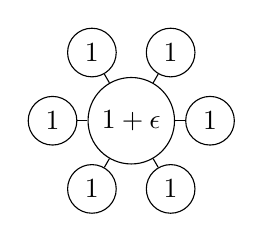
\begin{tikzpicture}
  \node[draw,circle] (G-1) at (0,0) {$1+\epsilon$};
  \node[draw,circle] (G-2) at (1,0) {1};
  \node[draw,circle] (G-3) at (0.5,0.866) {1};
  \node[draw,circle] (G-4) at (-0.5,0.866) {1};
  \node[draw,circle] (G-5) at (-1,0) {1};
  \node[draw,circle] (G-6) at (-0.5,-0.866) {1};
  \node[draw,circle] (G-7) at (0.5,-0.866) {1};
  \draw (G-1) -- (G-2);
  \draw (G-1) -- (G-3);
  \draw (G-1) -- (G-4);
  \draw (G-1) -- (G-5);
  \draw (G-1) -- (G-6);
  \draw (G-1) -- (G-7);
\end{tikzpicture}
\end{ex}
%TODO add the rest

\marginpar{Lecture 19}
%TODO add the rest


\marginpar{Lecture 20}

\section{Matroids}

\begin{defn}
Take a ground set $\X$ and a nonempty collection of subsets of $\X$ called $\I$.
If given $A\in \I,\ B\subseteq A$ then $B\in \I$, then we call the sets in $\I$ \emph{independent}.\\
And we then call $(\X,\I)$ an independence system.
\end{defn}

\begin{defn}
Given an independence system $(\X,\I)$ we call it a \emph{matroid} if 
$$A,B\in \I \text{ with } |A|<|B|, \text{ then } \exists x\in B\setminus A \text{ s.t. } A\cup \{x\} \in \I$$
\end{defn}

\begin{defns}
We say a set $B$ is a \emph{base} of $(\X,\I)$ if $B\in \I$ and $B\cup \{x\}\not\in\I\ \forall x\in\X\setminus B$.\\
All bases of a matroid have the same size.
This size is called the \emph{rank} of the matroid.
\end{defns}

We can also analogously define the base of a set $A\subseteq \X$ to be a maximal independent subset of $A$.

\begin{ex}
Given a graph $G = (V,E)$ we can take $\X = E$ and define $\I$ to be the set of forests in $G$.
This is clearly an independence system, so we just show that it is a matroid. \\
Suppose $A$ and $B$ are forests with $|A|<|B|$, then $B$ has fewer connected components than $A$.
So there is some $x\in B$ with endpoints in two different connected components of $A$ (by the pigeonhole principle).
So, $A\cup\{x\}$ must be a forest, so $A\cup\{x\} \in \I$. \\
The bases of this matroid are the spanning trees of the graph.
\end{ex}

\begin{ex}
Another historically important example of a matroid is a \emph{linear matroid} over a field $Q$.
Here $\X$ is a set of vectors in $Q^r$, and the independence system consists of independent sets of vectors.
\end{ex}

\begin{ex}
The \emph{uniform matroid} (of rank $k$) is defined an any ground set $\X$ by taking $\I$ to be all sets of at most $k$ elements from $\X$. 
\end{ex}

\begin{ex}
The \emph{partition matroid} is defined by taking a partition $\X_1,\X_2,\ldots,\X_m$ of $\X$, and non-negative integers $p_1,p_2,\ldots,p_m$ corresponding to the sets of the partition.
We then define $\I$ to be all the sets obtained by taking no more than $p_i$ elements from each $\X_i$.
\end{ex}

\begin{prop}
Let $\X$ be a ground set.
$\B$ is called the set of bases of a matroid if:
\begin{enumerate}
\item No set of $\B$ is contained in any other set of $\B$.
\item $\forall A,B\in\B$ and $x\in A\setminus B$, $\exists y\in B\setminus A$ s.t. $A\setminus\{x\}\cup\{y\} \in \B$.
\end{enumerate}
\end{prop}

\begin{proof}
(M$\cap$ I $\implies 1$): If any base $B\subset A$ then (M) says we can find $x\in A\setminus B$ s.t. $B\cup\{x\}\in \I$.
So $B$ is not a base, contradiction. \\
(M$\cap$ I $\implies 2$): Let A \& B be two bases of $(\X,\I)$ (note then we have $|A| = |B|$).
Let $x\in A\setminus B$.
Then $A' = (A\setminus\{x\})\in \I$, $|A'|<|A| = |B|$, so by (M) we can find $y\in B\setminus A' = B\setminus A$ s.t. $A'\cup \{y\}\in\I$.
Thus $A\setminus\{x\}\cup\{y\}\in\I$.
\end{proof} %TODO complete

\marginpar{Lecture 21}

\section{Max Spanning Trees}

\begin{alg}[Kruskal]~\\
Sort the edges $E$ into a list $e_1,\ldots,e_m$ by weight descending. \\
Let $S=\emptyset$ \\
For $i = 1$ to $m$:\\
\indent If $S\cup \{e_i\}$ does not contain a cycle then add $e_i$ to $S$.
\end{alg}

We can generalise this idea to other independence systems to get:

\begin{alg}[Standard greedy algorithm for independence system $\X,\I$]~\\
Sort the elements of $\X$ into a list $e_1,\ldots,e_m$ by weight descending. \\
Let $S=\emptyset$ \\
For $i = 1$ to $m$:\\
\indent If $S\cup \{e_i\}\in\I$ then add $e_i$ to $S$.
\end{alg}

When does this algorithm work?
It turns out this algorithm is optimal for an independence system $(\X,\I)$ iff the system is a matroid.

\begin{thm}
An independence system $(\X,\I)$ is a matroid iff (G), the standard greedy algorithm is optimal for all weight functions on $\X$.
\end{thm}

\begin{proof}
If $(\X,\I)$ is a matroid, then (G) holds.
We use the base characterisation.
(B2) if A and B are bases then for all $x\in B\setminus A$ $\exists y\in A\setminus B$ s.t. $A\setminus \{y\}\cup\{x\}$ is a base.
Let $w$ be an arbitrary function $w\colon \X \to \RR$ and $\OPT\in \I$ with $w(\OPT)$ maximum, and $G$ be a solution produced by the standard greedy algorithm.
Order the elements of OPT and $G$ by non-increasing weight.
Suppose that OPT and $G$ agree on $i$ elements and let $g$ be the first element they disagree on.
$\exists x \in \OPT$ s.t. $\OPT'=(\OPT \setminus \{x\}) \cup \{g\}\in\I$.
Let $C=\OPT\cap G$.
$$C\cup\{x\}\in \I,\ C\cup\{g\} \in \I\ \text{ and } w(x)\le w(g)$$
$$w(\OPT') $$
\end{proof}

%TODO finish all that....

\marginpar{Lecture 22}

\section{Graph Colourings}

\begin{defns}
A \emph{vertex $k$-colouring} is an assignment $f\colon V(G)\to C=\{1,\ldots,k\}$ from its vertex set onto the set of colours $C$ whose elements are called colours. \\
A vertex colouring is called \emph{proper} (or \emph{feasible}) if the endpoints for any edge are assigned different colours.\\
A \emph{colour class} is a set of vertices coloured with the same colour. \\
The \emph{vertex chromatic number} (or \emph{index}) of a graph $G$, denoted $\chi(G)$, is the minimum number of different colours required for a proper vertex colouring of $G$. \\
A graph $G$ is called $k$-vertex colourable if $\chi(G) = k$.
\end{defns}

\begin{alg}[Sequential (or Greedy)]~\\
\textbf{Input} a graph with vertex set $v_1,\ldots,v_n$. \\
\textbf{Output} a proper vertex colouring $f\colon V(G)\to \{1,\ldots,k\}$. \\
For $i = 1$ to $n$ \\
\indent Let $f(v_i)$ be the smallest colour number not used by any neighbours of $v_i$ with smaller index. \\
Return $f$.
\end{alg}

\begin{prop}
Let $G$ be a graph that has $k$ mutually adjacent vertices, then $\chi(G) \ge k$.
\end{prop}

\begin{defns}
A \emph{clique} in graph $G$ is a maximal subset of $V(G)$ whose vertices are mutually adjacent. \\
The \emph{clique number} $\omega(G)$ of $G$ is the number of vertices in the largest (maximum) clique in $G$.
\end{defns}

\begin{prop}
For any graph $\chi(G) \ge \omega(G)$.
\end{prop}

\begin{defn}
The \emph{independence number} $\alpha(G)$ of a graph $G$ is the number of vertices in an independent set of maximum cardinality.
\end{defn}

\begin{prop}
For any graph $G$, $\chi(G) \ge \left[ \frac{|V(G)|}{\alpha(G)}\right]$
\end{prop}

\begin{ex}
%TODO insert
\end{ex}

\begin{prop}
Let $H$ be a subgraph of $G$, then $\chi(G) \ge \chi(H)$.
\end{prop}

\begin{defn}
The join $G+H$ of two graphs $G$ and $H$ is obtained from $G\cup H$ by adding all edges between $V(G)$ and $V(H)$.
\end{defn}

\begin{prop}
$\chi(G+H) = \chi(G) + \chi(H)$.
\end{prop}

\begin{proof}
In the graph $G+H$ no colour used to colour $V(G)$ can be used for colouring $V(H)$ and conversely no colour used to colour $V(H)$ can be used to colour $V(G)$.
Therefore $\chi(G+H) \ge \chi(G) + \chi(H)$.
Colour $V(G)$ using proper colouring with colours $\{1,\ldots,\chi(G)\}$ and colour $V(H)$ using colours $\{\chi(G) + 1,\ldots, \chi(G) + \chi(H)\}$.
Therefore $\chi(G+H) \le \chi(G)  + \chi(H) $.
\end{proof}

\begin{prop}
\begin{enumerate}
\item A bipartite graph $G$ has $\chi(G) = 2$.
\item Path graphs $\chi(P_n) = 2$ for $n \ge 2$.
\item $\chi(T) = 2$ for any non-trivial tree (as trees are actually bipartite graphs).
\item For the hypercube graph $Q_n$, $\chi(Q_n) \le n$.
\item For even cycles $C_{2n}$ we have $\chi(C_{2n}) = 2$ (as bipartite).
\item For an odd cycle $C_{2n+1}$ we have $\chi(C_{2n+1}) = 3$.
\end{enumerate}
\end{prop}

\begin{proof}[Proof (of 6)]
$\chi(C_{2n+1}) \ge \left[ \frac{|V(G)|}{\alpha(G)}\right] = \left[\frac{2n+1}{n} \right] = 3$.
\end{proof}

\marginpar{Lecture 23}

\section{Brooks Theorem}

\begin{defns}
A \emph{block} is a maximal connected subgraph $H$ s.t. no vertex of $H$ is a cut vertex of $H$. \\
A \emph{leaf block} of a graph $G$ is a block that contains exactly one cut vertex of $G$.
\end{defns}

\begin{ex}
%TODO input
\end{ex}

\begin{prop}
Two different blocks of a graph have at most once vertex in common.
\end{prop}

\begin{prop}
Let $B_1$ and $B_2$ be two distinct blocks of a connected graph.
Let $y_1\in B_1$ and $y_2\in B_2$ be vertices that are not cut vertices in $G$.
Then $y_1$ is not adjacent to $y_2$.
\end{prop}

\begin{prop}
A graph with at least one cut-vertex has at least two blocks.
\end{prop}

\begin{lem}
Let $G$ be a non-complete $k$-regular 2-connected graph with $k \ge 3$.
Then $G$ has a vertex $x$ with two non-adjacent neighbours $y$ and $z$ s.t. $G\setminus \{y,z\}$ is a connected graph.
\end{lem}

\begin{proof}
Let $w$ be any vertex in $G$. If $G\setminus\{w\}$ is 2-connected then let $z$ be ant vertex at distance 2 from $w$.
If $x$ is the vertex between $w$ and $z$ and $y = w$ then the conditions of the lemma are satisfied. \\
Alternatively assume $k_V(G\setminus w) = 1$.
Then let $B_1$ and $B_2$ we two leaf blocks of $G\setminus w$.
Since $G$ has no cut vertices we know that $w$ must be adjacent to some vertex $y_1 \in B_1$ which is not a cut vertex of $G\setminus w$ and it should be adjacent to some $y_2 \in B_2$ that is no a cut vertex of $G\setminus w$.
By the above proposition $y_1$ is not adjacent to $y_2$.
We define $x = w$, $y = y_1$, $z = y_2$.
\end{proof}

\begin{thm}[Brooks]
Let $G$ be a non-complete connected graph with maximum degree $\Delta(G) \ge 3$.
Then $\chi(G) \le \Delta(G)$.
\end{thm}

\begin{proof}
\textbf{Case 1} $G$ is not regular.
Let $n = |V(G)|$.
Choose $v_n$ to be any vertex of degree less than $\Delta(G)$.
Next grow a spanning tree from $v_n$, assigning indices in decreasing order.
Apply a sequential greedy algorithm to the ordering $v_1,\ldots,v_n$. \\
\textbf{Case 2} $G$ is regular and $G$ has a cut-vertex $x$.
Let $C_1,\ldots, C_m$ be the components of $G\setminus x$.
Let $G_i$ be the subgraph induced by $C_i\cup x$.
The degree of $x$ in $G_i$ is $< \Delta(G)$.
Each $G_i$ has a proper colouring with $\Delta(G)$ colours.
By permuting colour classes we can ensure that vertex $x$ is coloured using the same colour in all $G_i$.
Therefore we can continue colourings of $G_i$ into a proper colouring of $G$. \\
\textbf{Case 3} $G$ is regular and 2-connected.
By the previous lemma, $G$ has a vertex $v_n$ with two non-adjacent neighbours $v_1, v_2$ s.t. $G\setminus\{v_1,v_2\}$ is connected.
Grow a spanning tree in $G\setminus \{v_1,v_2\}$ starting from $v_n$ assigning indices in decreasing order.
The sequential algorithm will use at most $\Delta(G)$ colours for $v_3,\ldots, v_{n-1}$, we can use the same colour for $v_1$ and $v_2$.
Therefore $\Delta(G)$ colours is feasible for $v_n$.
\end{proof}

\marginpar{Lecture 24}

\section{Edge-colouring}

\begin{defns}
An \emph{edge $k$-colouring} is an assignment $f\colon E(G) \to C$ from its edge set onto the set $C=\{1,\ldots, k\}$ (or indeed any set of cardinality $k$), whose elements are called colours. \\
An \emph{edge colour class} is a subset of $E(G)$ in which all edges have the same colour. \\
A \emph{proper edge colouring} of a graph is an edge colouring such that adjacent edges are assigned different colours. \\
The \emph{edge chromatic number} of $G$ is denoted by $\chi'(G)$ is the minimum number of different colours required for a proper edge-colouring of $G$.
\end{defns}

\begin{ex}
Matching teachers to classes where they can't be matched to two at the same time is an example of bipartite graph colouring.
\end{ex}

\begin{prop}
Let $\alpha'(G)$ be the cardinality of a maximum matching in $G$, then $\chi'(G) \ge \lceil\frac{|V(G)|}{\alpha'(G)}\rceil$.
\end{prop}

\begin{defns}
The \emph{chromatic incidence} at vertex $v$ of a given edge colouring $f$ is the number of different edge colours incident on $v$.
It is denoted $\ecr_v(f)$.\\
The \emph{total chromatic incidence} for an edge colouring $f$ of $G$ is $\ecr(f) = \sum_{v\in V(G)} \ecr_v(f)$.
\end{defns}

\begin{prop}
An edge colouring $f$ of $G$ is proper $\iff$ for all $v\in V(G)$ we have $\ecr_v(f) = d_v$ (the degree of $v$).
\end{prop}

\begin{defn}
A \emph{Kempe $i$-$j$ edge-chain} is a component of the subgraph of $G$ induced on all edges coloured $i$ and $j$.
\end{defn}

A slightly clearer definition, courtesy of Wikipedia:
\begin{defn}
Let $G$ be a graph $G$ with a particular edge colouring.
For an edge $e \in E(G)$ which is coloured $i$, the \emph{Kempe $i$-$j$ edge-chain of $G$ containing $e$} is the maximal connected subset of $E(G)$ containing $e$ and all other edges which are coloured either $i$ or $j$.
\end{defn}
\begin{ex}
An edge 4-colouring, with the two Kempe 1-2 edge chains shown as dashed edges.
$$
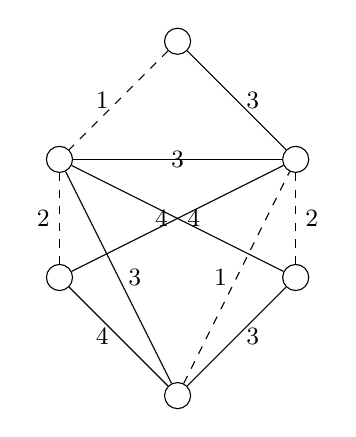
\begin{tikzpicture}[baseline=5.5ex]
  \tikzstyle{every node}=[font=\small]
  \node[draw,circle] (1) at (1.5,4.5) {};
  \node[draw,circle] (2) at (0,3) {};
  \node[draw,circle] (3) at (3,3) {};
  \node[draw,circle] (4) at (0,1.5) {};
  \node[draw,circle] (5) at (3,1.5) {};
  \node[draw,circle] (6) at (1.5,0) {};
  \path[]
  (1) edge node [right]{3} (3)
    (2) edge node {3} (3)
    (3) edge node [left]{4} (4)
    (4) edge node [left]{4} (6)
    (5) edge node [right]{4} (2)
    (6) edge node [right]{3} (5)
    (2) edge node [right]{3} (6);
  \draw[dashed]
  (1) edge node [left]{1} (2)
  (2) edge node [left]{2} (4)
  (6) edge node [left]{1} (3)
    (3) edge node [right]{2} (5);
\end{tikzpicture}
$$
%TODO: Examples
\end{ex}

\begin{lem}
Let $f$ be an edge $k$-colouring of $G$ with the largest possible chromatic incidence.
Let $v$ be a vertex on which some colour $i$ is incident at least twice and on which some colour $j$ is not incident at all.
Then a Kempe $i$-$j$ chain containing $v$ is an odd cycle.
\end{lem}

Proof later.

\begin{lem}
Let $G$ be a connected graph with at least two edges that is not an odd-cycle graph.
Then $G$ has an edge-colouring such that both colours are incident on every vertex of degree at least 2.
\end{lem}

\begin{proof}
We have three cases:
\begin{itemize}
\item Even cycle
\item Not a cycle but Eulerian
\item Not Eulerian
\end{itemize}
\end{proof}

\begin{proof}[Proof of first lemma]
Assume it is not an odd cycle - then we are in the case of the second lemma.
So each vertex will get at least two colours.
So we can increase the chromatic incidence, but this is a contradiction, so it is an odd cycle.
\end{proof}

\begin{thm}[K\"onig]
Let $G$ be a bipartite graph.
Then $\chi'(G) = \Delta(G)$ (maximal degree).
\end{thm}

\begin{proof}
Suppose $\chi'(G) \ne \Delta(G)$.
Then $\Delta(G) < \chi'(G)$ (as we know $\Delta(G) \le \chi'(G)$ always).
Let $f$ be an edge $\Delta$-colouring of $G$ for which $\ecr(f)$ is maximised.
Since $f$ is not proper $\exists v\in V(G)$ such that $\ecr_v(f) < d_v$.
Thus some colour occurs on at least two edges incident on $v$.
Since there are $\Delta$ colours in total, and at most $\Delta-2$ remaining edges incident on $v$, there should be some colour not incident on $v$.
By previous lemma the graph $G$ contains an odd cycle, this is a contradiction with $G$ being bipartite.
\end{proof}

\begin{thm}[Vizing]
Let $G$ be a simple graph.
Then there exists a proper edge colouring of $G$ using less than $\Delta(G) + 1$ colours.
\end{thm}

(It is actually NP hard to show whether your graph will need $\Delta(G)$ or $\Delta(G) + 1$ colours.)

%TODO some more stuff here maybes

\marginpar{Lecture 25} 

\section{Tree width}

We define the tree decomposition $T$ of a graph $G$ as follows: \\
$T$ has vertices $i$ labelled with sets $X_i$ of vertices from $G$, satisfying:
\begin{enumerate}
\item $T$ is a tree.
\item For every edge $(u,v)\in E(G)\ \exists$ a vertex in $T$ with both $u$ and $v$ in its set.
\item For all $X_i,X_j,X_k\in V(T)$ if $X_j$ is on the path from $X_i$ to $X_k$ then $X_i\cap X_k\subseteq X_j$. In other words, if $X_i$ and $X_k$ both contain a vertex $v$, then all vertices $X_j$ of the tree in the (unique) path between $X_i$ and $X_j$ contain $v$ as well. This is known as the `running intersection property' (Diestel, 2005).
\end{enumerate}

\begin{ex}
%TODO like every other example lols.
\end{ex}

\begin{defn}
The \emph{tree width} of a tree decomposition $T$ is the maximum size of a label set $- 1$:
$$\max_{i\in V(T)} \{|X_i| -1\}$$
The \emph{tree width} a graph $G$ is defined to be the minimum tree width of any tree decomposition of $G$.
\end{defn}

\begin{thm}
Every tree has tree width 1.
\end{thm}

\begin{proof}[Proof sketch]
\begin{itemize}
\item Pick a root.
\item Put a vertex for every parent and child.
\end{itemize}
\end{proof}

\begin{lem}
If there is a tree decomposition with tree width $k$ then there is one $T$ that satisfies $\forall i, j\in V(T)\ X_i\not\subseteq X_j$.
\end{lem}

\begin{proof}
Let $X_i\subseteq X_j$, and $X_k\supseteq X_i\cap X_j = X_i$.
Now delete $X_i$. \\
%Assume this is not a tree decomposition but TODO make sure this acutally makes sense
\end{proof}

\begin{lem}
Every clique of size $n$ has tree width at least $n-1$.
\end{lem}

\begin{proof}
Suppose there is a tree decomposition of width $\le n-2$ for $K_n$.
By the above lemma all $X_i$ must be missing at least one vertex of $K_n$.
If $I$ has only one vertex $i$ in $T$, then $I$ does not have edges in the vertex of $G$ missing from $X_k$.
So $I$ must have at lest two vertices (say $i$ \& $j$).
There is some $v\in V(G)$ s.t. $v\not\in X_i$.
$X_j \not\subseteq X_i$, $X_i$ has a vertex $v\not\in X_j$.
$X_i \not\subseteq X_i$, $X_j$ has a vertex $v\not\in X_i$.
So $\{v,u\} \not\in X_i$, $\{v,u\} \not\in X_j$ but $\{v,u\}\in E(K_n)$.
$\exists X_k$ s.t. $v,u\in X_k$ but $X_k$ needs to connect to $X_i \& X_j \implies $ a cycle, not a tree.
So the tree width is $n-1$. %TODO make this make sense too
\end{proof}

\begin{ex}
Consider $C_6$:
\begin{center}
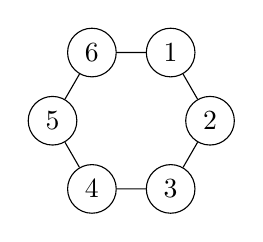
\begin{tikzpicture}
  \node[draw,circle] (G-1) at (1,0) {2};
  \node[draw,circle] (G-2) at (0.5,0.866) {1};
  \node[draw,circle] (G-3) at (-0.5,0.866) {6};
  \node[draw,circle] (G-4) at (-1,0) {5};
  \node[draw,circle] (G-5) at (-0.5,-0.866) {4};
  \node[draw,circle] (G-6) at (0.5,-0.866) {3};
  \draw (G-1) -- (G-2) -- (G-3) -- (G-4)  -- (G-5)  -- (G-6) -- (G-1);
\end{tikzpicture}
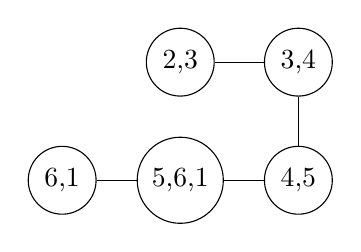
\begin{tikzpicture}
  \node[draw,circle] (G-1) at (-1.5,0) {6,1};
  \node[draw,circle] (G-2) at (0,0) {5,6,1};
  \node[draw,circle] (G-3) at (1.5,0) {4,5};
  \node[draw,circle] (G-4) at (1.5,1.5) {3,4};
  \node[draw,circle] (G-5) at (0,1.5) {2,3};
  \draw (G-1) -- (G-2) -- (G-3) -- (G-4)  -- (G-5);
\end{tikzpicture}
\end{center}
\end{ex}

By restricting to graphs with bounded tree width (that is at most $k$ for some constant $k$) we can find exact algorithms for a large class of problems that take $O(n)$ time.

%\section{Max independent set for trees} TODO whole section yawn

\section{Monadic second order logic}

\begin{thm}[Courcelle]
Any property that can be expressed in Monadic second order logic can be tested in time $f(k,p)\cdot O(n)$ on graphs of tree width $\le k$.
Where $p$ is the size of the monadic second order logic property, $n = |V|$ and $k$ is the tree width.
\end{thm}

We have a few :
\begin{itemize}
\item Relations $R(x,y)$
\item Conjectures $\neg,\implies,\vee,\wedge$
\item Equality
\end{itemize}

First order logic has $\forall$ and $\exists$ that can be used to quantify elements of the universe.\\
Second order logic can quantify elements of the universe and relations on them, e.g. $\forall R\ \exists x\ \exists y$ s.t. $R(x,y)$. \\
Monadic second order logic can quantify over elements of the universe and only sets (relations with only one element) are allowed.

%\begin{thm}
%We can also test that $\exists S\in 
%\end{thm}

\end{document}
